\documentclass{article}

\usepackage[utf8]{inputenc}
\usepackage{natbib}
\usepackage{tabularx} % tables, auto-width
\usepackage{float} % figure 'H' option
\usepackage{changepage} % adjustwidth
\usepackage{syntax} % grammar
\usepackage{minted} % JSON syntax
\usepackage{tikz-qtree} % trees, multiline node names
\usepackage{enumitem} % begin list at 0
\usepackage{multicol} % comparing adjacent semantics
% \usepackage{microtype}

\setminted{samepage}

\begin{document}

\title{A Natural Language Interface for Querying
Graph-Structured Data}
\author{Danny Nemer\\
Washington University in St. Louis\\
\texttt{danny.nemer@wustl.edu}}
\date{May 2015}
\maketitle


\begin{abstract}
This paper proposes a robust natural language interface (NLI) for querying graph-structured data. In addition to parsing text, the NLI sophisticatedly handles ill-formed input, auto-completes queries as they are input, and displays the \textit{k}-best interpretations of the input query as suggestions.

The system displays suggested queries as the user types, demonstrating to the user that it correctly understands the input before the user attempts to execute a search. The auto-completion also accelerates user input. In contrast, most NLIs today require the user to submit input and wait for the parser to report if it successfully understands, leading to high failure rates of user interaction.

Furthermore, the grammar for the parser is as robust as the English language permits. If the database behind the interface holds the data being queried, then the NLI will understand every possible variant of a query that is within reason. As a result, the interface is accessible to any speaker of the English language; yet, it makes no sacrifices in its ability to understand the precise intention of the user.
\end{abstract}


\section{Introduction}
Searching a vast graph of structured data, such as a relational database, is challenging. Consider a database where each entry represents a node, and relations between the entries represent edges. Each entry also holds structured information, which is the node's properties. The working example for this paper will be LinkedIn's database of professionals. Entries (nodes) are users, companies, industries, cities, et cetera. Each entry can have relations (edges) to others, such as users that are employees of a company, or a company that operates in a specific industry and city. Each entry has properties such as a user's name, dates of employment, or degrees held.

A query interface for searching this complex graph must understand the user's intent precisely. One possible interface is keyword-based search; however, the ability to understand the user's intent is limited. For example, ``\textit{people St.\ Louis}'' can mean ``\textit{people who live in St. Louis}'', ``\textit{people who work in St.\ Louis}'', or ``\textit{people who have worked or lived in St.\ Louis}''. Another possible interface is a filter-based form of checkboxes and drop-down selections; however, the interface becomes too complicated and inefficient when implemented to support hundreds of different filters for nodes and edges. The simplest and most efficient interface for querying a complex graph of structured data is a natural language interface. For example:
\begin{quote}
\textit{Computer scientists I am connected to who work with people who graduated from my college last year and do not live in St.\ Louis}
\end{quote}
Such a system must be absolutely robust. This entails handling ill-formed queries (including traditional keyword searches not in the form of a proper query) and queries that have different linguistic forms but are semantically identical.

The proposed interface parses the user's input and outputs the \textit{k}-best suggestions in natural language. For example:
\begin{quote}
\textit{people who work nearby}\\
output:\\
\texttt{
People who work nearby\\
People who work nearby from St.\ Louis\\
Connections of people who work nearby\\
People who work nearby and work at Washington University in St.\ Louis
}
\end{quote}
Each suggestion expresses the system's interpretation of the user's exact intention. The system's ability to output the \textit{k}-best suggestions instantly as the user types allows the user to know whether their query has been correctly understood before he or she executes the search. The user also knows the parser will correctly interpret any suggestion the user chooses, even if it does not match the input, as with ill-formed input:
\begin{quote}\textit{people who nearby}\\
output:\\
\texttt{
People who live nearby\\
People who work nearby\\
People who work near Washington University in St.\ Louis\\
People who work nearby and live in St.\ Louis
}
\end{quote}
\begin{quote}
\textit{people me is connect to}\\
output:\\
\texttt{
People I am connected to\\
People my connections are connected to\\
People I am connected to who work nearby\\
People I am connected to who live nearby
}
\end{quote}
This solves a common problem of natural language interfaces: the user does not know if an interaction (i.e., input) is successful until after execution, which can consume more time than the manual alternative if the parser fails. The output also includes suggestions for completing the search as it is being input, providing a real-time experience:
\begin{quote}
\textit{people wh}\\
output:\\
\texttt{
People who I am connected to\\
People who attend Washington University in St.\ Louis\\
People who work at Washington University in St.\ Louis\\
People who live in St.\ Louis
}
\end{quote}
The auto-completion demonstrates what queries are possible and allows the user to accelerate his or her input.

While this system is introduced in the frame of searching complex graphs, additional natural language interfaces can be built with it. For example, productivity software can leverage the system: ``\textit{schedule a meeting with John every Tuesday at 4:00 in the afternoon}'', and ``\textit{remind me to take out the trash at sundown}''. Searching complex graphs, however, is the most important and challenging problem this project attempts to solve.


\section{Grammar}
\subsection{Design}
A weighted context free grammar (WCFG) defines the queries that the parser can understand. WCFGs are an extension of context free grammars (CFG), as formalized by Chomsky \citep{Chomsky1956}, with numeric weights assigned to each production. The grammar is composed of production rules that recursively generate expressions from symbols, as shown in the example grammar in Figure \ref{fig:grammar}.

\begin{figure}[H]
\begin{adjustwidth}{4.1em}{4.1em}
\setlength{\grammarindent}{11em}
\begin{grammar}
<start> ::= <users>

<users> ::= <people> <user-filter>

<user-filter> ::= <who> <employer-filter>
\alt <who> <residence-filter>

<employer-filter> ::= <work-current> <employer-location>
\alt <work-current> <employer-subject>

<residence-filter> ::= <live-in> <location>

<employer-location> ::= <in-work> <location>

<employer-subject> ::= <at-work> <employer>

<location> ::= <city>

<employer> ::= \{employer\}

<city> ::= \{city\}

<people> ::= `people'

<who> ::= `who'
\alt `that'

<work-current> ::= `work'

<in-work> ::= `in'
\alt `around'

<at-work> ::= `at'
\alt `for'

<live-in> ::= `live in'
\end{grammar}
\end{adjustwidth}
\caption{A simplified natural language CFG.}
\label{fig:grammar}
\end{figure}

The left-hand-side of each rule is a single non-terminal symbol, which produces a terminal symbol or a string of non-terminal symbols on the right-hand-side. A terminal symbol is an item the parser will expect to see in its input. This can be a word or phrase, including \lit{people}, \lit{live in}, and \lit{work}; or it can be an entity, including \texttt{\string{employer\string}} and \texttt{\string{city\string}}.

The parser uses the grammar's rules to construct a parse tree from an input query. A parse tree's construction begins at the \synt{start} symbol, and recursively expands the production rules until it halts upon reaching terminal symbols, as shown in Figure \ref{fig:parsetree}.

\begin{figure}[H]
\centering
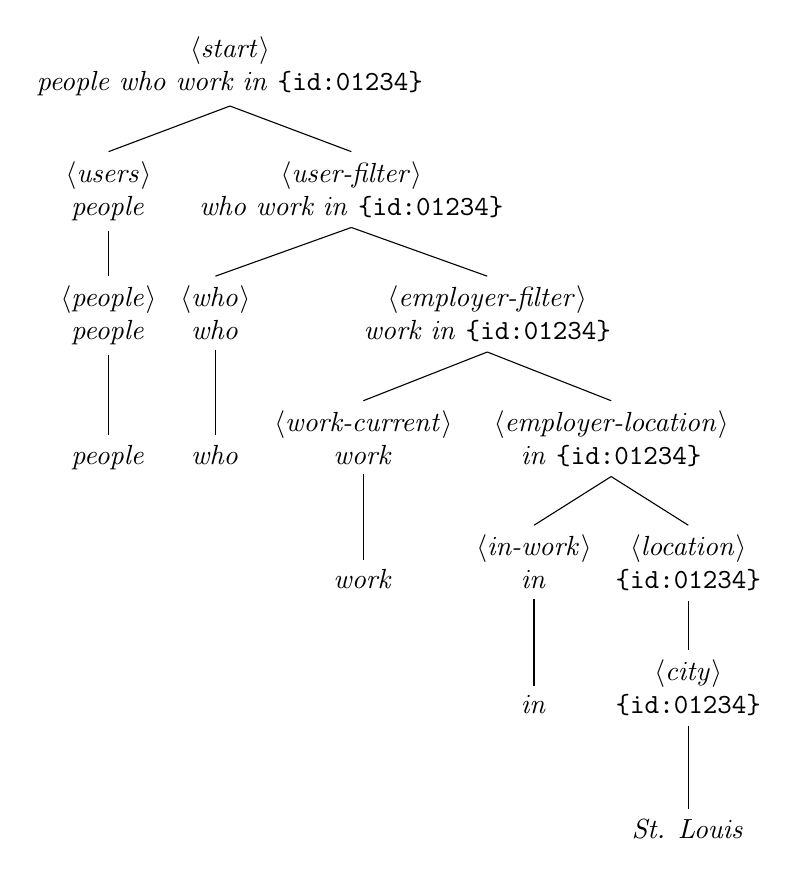
\begin{tikzpicture}[align=center, level distance=45pt]
\Tree
[.\node{\synt{start}\\\textit{people who work in} \texttt{\string{id:01234\string}}};
    [.\node{\synt{users}\\\textit{people}};
        [.\node{\synt{people}\\\textit{people}};
            \textit{people}
        ]
    ]
    [.\node{\synt{user-filter}\\\textit{who work in} \texttt{\string{id:01234\string}}};
        [.\node{\synt{who}\\\textit{who}};
            \textit{who}
        ]
        [.\node{\synt{employer-filter}\\\textit{work in} \texttt{\string{id:01234\string}}};
            [.\node{\synt{work-current}\\\textit{work}};
                \textit{work}
            ]
            [.\node{\synt{employer-location}\\\textit{in} \texttt{\string{id:01234\string}}};
                [.\node{\synt{in-work}\\\textit{in}};
                    \textit{in}
                ]
                [.\node{\synt{location}\\\texttt{\string{id:01234\string}}};
                    [.\node{\synt{city}\\\texttt{\string{id:01234\string}}};
                        \textit{St. Louis}
                    ]
                ]
            ]
        ]
    ]
]
\end{tikzpicture}
\caption{A parse tree constructed from the grammar in Figure \ref{fig:grammar}.}
\label{fig:parsetree}
\end{figure}

\subsection{Semantics}
Each production rule can contain numerous properties in addition to the right-hand-side symbol(s) it produces. One such property is a semantic representation of that rule in the form of a semantic function. A semantic function is a computer-readable instruction that can be executed against a database to perform a search. For example, in the parse tree in Figure \ref{fig:parsetree}, the rule produced by \synt{employer-location} is associated with the semantic \texttt{employer-location}.

A semantic function can accept arguments such as an entity ID or other semantic functions. Hence, a parse tree whose construction includes multiple rules with one or more semantic functions will produce a semantic representation of the entire tree. As a result, the parse tree in Figure \ref{fig:parsetree} will generate the following semantic:
\begin{quote}
\begin{minted}{js}
present: [ {
  employees: [ {
    employer-location: [ 01234 ]
  } ]
} ]
\end{minted}
\end{quote}
In this semantic, \texttt{01234} is the ID of the St. Louis \texttt{\string{city\string}} entity. The entire semantic can be executed against a database.

\subsection{Costs}
The grammar uses a cost parametrization, assigned to production rules as weights,  to rank parse trees:
\begin{enumerate}
\item Semantic costs: Every semantic function has an associated cost. Thus, the more complex a query suggestion is, translating to a complex semantic representation, the greater the cost associated with it is. These costs are assigned to the grammar and therefore independent of input.
\item Display text costs: Several terminal symbols, which constitute a query suggestion's display text, have cost penalties derived from their length and likelihood. A precise phrase such as \lit{residents of} will have a higher cost than the common preposition \lit{by}. These costs are assigned to the grammar and therefore also independent of input.
\item Entity costs: Each matching of input text with an entity, such as ``\textit{NYC}'' with \texttt{\string{city\string}}, produces a cost based on the quality of the match.
\item Edit costs: In order to produce the \textit{k}-best interpretations of an input query, the parser considers four edit operations to the input that can produce viable suggestions. Each instance of an edit, as shown in the table below, has an associated cost. This category of costs is the most influential in the relative ranking of parse trees.\\\\
\begin{tabularx}{\linewidth}{ l X X }
& Input & Output\\
Insertion & \textit{connections St.\ Louis} & \texttt{my connections who live in St.\ Louis}\\
Deletion & \textit{who are my connections working in St.\ Louis} & \texttt{my connections who work in St.\ Louis}\\
Transposition & \textit{Wash U students} & \texttt{students of Washington University}\\
Substitution & \textit{me friends at Wash U} & \texttt{my connections who attend Washington University}
\end{tabularx}
\end{enumerate}


\section{Robustness}
The grammar for this system is designed to be as robust as possible, allowing a user to phrase a query in various ways, even if the input is ill-formed. For example, the following are all semantically equivalent, and exemplify the diverse phrasing understood by the parser:
\begin{itemize}
\item \textit{people who go to my college}
\item \textit{current students of my college}
\item \textit{people who are studying at the college of mine}
\item \textit{people who have been attending my university}
\end{itemize}
This also extends to ill-formed queries:
\begin{itemize}
\item \textit{people that attends mine college}
\item \textit{person who is at the university of me}
\end{itemize}
When parsed, all of these queries are translated to the same semantic:
\begin{quote}
\begin{minted}{js}
present: [ {
  students: [ {
    colleges-attended: [ me ]
  } ]
} ]
\end{minted}
\end{quote}
Ultimately, the parser aims to generate plausible suggestions for any reasonable input.

\subsection{Synonyms}
One of the methods by which the natural language interface achieves its vast scope of understanding is with synonyms. Each terminal rule has several synonymic terminal symbols. For example:
\begin{quote}
\setlength{\grammarindent}{8em}
\begin{grammar}
<college-term> := `college'
\alt `university'
\alt `school'
\end{grammar}
\end{quote}
Here, \synt{college-term} accepts three different terms. Additional specifications in the grammar instruct the parser to accept two of these terms, \lit{college} and \lit{university}, but to replace \lit{school} with \lit{college} when seen in input, as it is ill-fit for the parse trees built with \synt{college-term}. The latter case, which replaces the input text, is an instance of a substitution edit and therefore has a cost penalty.

\subsection{Inflections}
Morphological analysis accounts for the inflected forms of the words in the grammar's terminal rules. This ensures output suggestions are always in grammatical agreement, irrespective of the correctness of input. Some inflections do not change meaning, e.g., \lit{employer} and \lit{employers}, while others do, e.g., ``\texttt{people who attend \string{college\string}}'' opposed to ``\texttt{people who attended \string{college\string}}''. Specifically, the grammar considers the following cases:
\begin{enumerate}
\item Grammatical case:
\begin{enumerate}
\item Nominative: \textit{people \textbf{me} am connected to} $\rightarrow$    \texttt{people} \bfseries I \mdseries \texttt{am connected to}
\item Objective: \textit{people connected to \textbf{I}} $\rightarrow$ \texttt{people connected to} \bfseries me \mdseries
\end{enumerate}
\item Verb form:
\begin{enumerate}
\item Tense: \textit{people who have \textbf{attend} college} $\rightarrow$ \texttt{people who have} \bfseries attended \mdseries \texttt{college}
\item Voice: \textit{schools \textbf{attend} by my former colleagues} $\rightarrow$ \texttt{schools} \bfseries attended \mdseries \texttt{by my former colleagues}
\end{enumerate}
\item Person-number:
\begin{enumerate}
\item First-person-singular: \textit{people I \textbf{are} connected to} $\rightarrow$ \texttt{people I} \bfseries am \mdseries \texttt{connected to}
\item Third-person-singular: \textit{colleges \{user\} \textbf{attend}} $\rightarrow$ \texttt{colleges \string{user\string}} \bfseries attends \mdseries
\item Third-person-plural: \textit{people who \textbf{goes} to my college} $\rightarrow$ \texttt{people who} \bfseries go \mdseries \texttt{to my college}
\item Plural: \textit{colleges I and \{user\} \textbf{attends}} $\rightarrow$ \texttt{colleges I and \string{user\string}} \bfseries attend \mdseries
\end{enumerate}
\end{enumerate}

\subsection{Optional terms}
In order to extract the meaningful portions of a query for the parser, particular words are identified as optional in particular contexts:
\begin{itemize}
\item \textit{people who have lived in St. Louis} $\rightarrow$ \texttt{people who lived in St.\ Louis}
\item \textit{the companies that I work for} $\rightarrow$ \texttt{companies I work for}
\end{itemize}
In the second example, ``\textit{the}'' is disregarded when preceding the head noun in ``\textit{the companies}''. The term should not be disregarded in other contexts, however, such as ``\textit{people who work in the}'', which can be completed to ``\textit{people who work in theater}''.


\section{Parser}
\subsection{GLR shift-reduce parsing}
The parser is an implementation of the Generalized Left-to-right Rightmost-deviation (GLR) parsing algorithm, formalized by Lang \citep{Lang1974}. GLR itself is an extension of Knuth's LR parsing algorithm \citep{Knuth1965} to handle nondeterministic, cyclic, and ambiguous context free grammars, as is the case for natural language grammars. It has a worst-case time complexity of $O(n^3)$, where \textit{n} is the number of input tokens (i.e., symbols). Unlike traditional LR parses, GLR uses breadth-first search to handle all possible interpretations of a given input.

\begin{figure}[h!]
\begin{adjustwidth}{3.6em}{3.6em}
\begin{enumerate}[start=0, label=\arabic*:]
\item \synt{start} $\Rightarrow$ 1\\
    \synt{users-start} $\Rightarrow$ 2\\
    \synt{people} $\Rightarrow$ 3
\item accept
\item {[} \synt{start} $\rightarrow$ \synt{users-start} ]
\item \synt{user-filter} $\Rightarrow$ 4\\
    \synt{who} $\Rightarrow$ 5
\item {[} \synt{users-start} $\rightarrow$ \synt{people} \synt{user-filter} ]
\item \synt{employer-filter} $\Rightarrow$ 6\\
    \synt{residence-filter} $\Rightarrow$ 7\\
    \synt{work-current} $\Rightarrow$ 8\\
    \synt{live-in} $\Rightarrow$ 9
\item {[} \synt{user-filter} $\rightarrow$ \synt{who} \synt{employer-filter} ]
\item {[} \synt{user-filter} $\rightarrow$ \synt{who} \synt{residence-filter} ]
\item \synt{employer-location} $\Rightarrow$ 10\\
    \synt{employer-subject} $\Rightarrow$ 11\\
    \synt{in-work} $\Rightarrow$ 12\\
    \synt{at-work} $\Rightarrow$ 13
\item \synt{location} $\Rightarrow$ 14\\
    \synt{city} $\Rightarrow$ 15
\item {[} \synt{employer-filter} $\rightarrow$ \synt{work-current} \synt{employer-location} ]
\item {[} \synt{employer-filter} $\rightarrow$ \synt{work-current} \synt{employer-subject} ]
\item \synt{location} $\Rightarrow$ 16\\
    \synt{city} $\Rightarrow$ 15
\item \synt{employer} $\Rightarrow$ 17
\item {[} \synt{residence-filter} $\rightarrow$ \synt{live-in} \synt{location} ]
\item {[} \synt{location} $\rightarrow$ \synt{city}]
\item {[} \synt{employer-location} $\rightarrow$ \synt{in-work} \synt{location} ]
\item {[} \synt{employer-subject} $\rightarrow$ \synt{at-work} \synt{employer} ]
\end{enumerate}
\end{adjustwidth}
\caption{A shift-reduce parse table generated from the grammar in Figure \ref{fig:grammar}.}
\label{fig:parsetable}
\end{figure}

Before parsing input, a shift-reduce parse table, a type of state transition table, is constructed from the context free grammar. The parse table, as shown in Figure \ref{fig:parsetable}, is a list of parsing states, each containing possible actions the parser can perform. State 1 in the table, which maps to `accept', is the accepting state of the parser that indicates the parse is successful and complete. Other states can contain shift or reduce steps:

\begin{itemize}
\item A shift step advances in the input query by one terminal symbol, which itself becomes a new single-node parse tree. This is modeled in the parse table in Figure \ref{fig:parsetable} as follows:
\begin{quote}
0: \synt{people} $\Rightarrow$ 3
\end{quote}
This action instructs a shift (or goto) on \synt{people} from state 0 to state 3.

\item A reduce step applies a completed production rule to previously constructed parse trees, merging them into one tree with a new root symbol. This is modeled in the parse table in Figure \ref{fig:parsetable} as follows:
\begin{quote}
4: {[} \synt{users-start} $\rightarrow$ \synt{people} \synt{user-filter} ]
\end{quote}
This action instructs a reduction whereby \synt{people} and \synt{user-filter} are combined into a new node of type \synt{users-start}.
\end{itemize}

Upon receiving input, the parser will process the input through a combination of shift and reduce steps, under the direction of the parse table. Each shift step is followed by a reduce step (i.e., reduction), which itself may have subsequent reductions. After completing all reductions specified in the parse table, the parser performs another shift step. The parser continues until it has processed the entire input.

While performing the reductions, the parser incrementally builds parse trees bottom-up (i.e., from terminal rules to the \synt{start} symbol) and left-to-right, without looking ahead (i.e., LR(0)) or backtracking (i.e., online). To be legal, a tree must reach the \synt{start} symbol and consist of consecutive, non-overlapping terminal symbols that comprise the entire input.

Given a state and input symbol, the parse table allows for multiple state transitions where traditional parse tables allow for only one transition. This allows for shift/reduce and reduce/reduce conflicts. When the parser encounters a conflicting transition, it forks the parse stack into two or more stacks. The previous node becomes a packed-node and the state corresponding to each possible transition becomes a sub-node and resides at the top of each of these stacks. The next shift step determines the next transition(s) for each of the sub-nodes, where further forking can occur. If the input symbol and a given sub-node's state do not have at least one possible transition (in the parse table), then the stack cannot produce a valid tree and is discarded.

The parsing algorithm is optimized by sharing common nodes in the parse stacks. When forking a stack, each packed-node shares identical parent and child nodes instead of duplicating the whole stack. This improvement produces a single parse forest, a directed acyclic graph-structured stack, rather than a set of individual parse trees, reducing memory requirements.

\subsection{Parse forest reduction}
The system then attempts to reduce the size of the parse forest output by the previous step. This entails reducing all unary branches within the forest, i.e., one symbol on the rule's right-hand-side that produce a single non-packed node. Specifically, an algorithm merges the rules' costs and any associated semantic functions, grammatical properties, edit properties, and display text. During this reduction, and in preparation of the system's next step, the algorithm also calculates the minimum cost of any sub-tree that can expand from each node in the parse forest.

\subsection{A* search}
Lastly, the system searches the parse forest for the \textit{k}-best parse trees, along with their semantic and textual representations. An \textit{n}-shortest path extension of the Hart \textit{et al.}'s A* search algorithm \citep{Hart1968} is used, which itself is an extension of Dijkstra's shortest path algorithm \citep{Dijkstra1959}, to traverse the parse forest. As each node in the parser forest is derived from a production rule in the grammar, the algorithm uses the rule's base costs and edit costs to rank the relative trees and sort the priority queue, which is a min-binary heap. In addition, the minimum cost of each sub-tree at each node, calculated in the previous forest-reduction step, is used as a heuristic to estimate the minimum cost to complete each tree from each node. This heuristic significantly accelerates computation.

\subsubsection{Grammatical conjugation}
While searching for the \textit{k}-best parse trees, the algorithm also constructs the associated display text of each tree. In addition to simple concatenation of terms, it accurately conjugates the text based both on the rules in which the terminal symbols are used, and on grammatical properties seen earlier in the tree. In the nominative case, for instance, a verb's inflection is derived from the person-number of the sentence's subject earlier in the parse tree:
\begin{quote}
\texttt{colleges \string{user\string} \synt{attend-term} $\rightarrow$ colleges \string{user\string} attends}
\end{quote}
Here, the conjugation of the terminal rule \synt{attend-term} $\rightarrow$ \lit{attends} depends on the previously seen third-person-singular property defined by \synt{users} $\rightarrow$ \texttt{\string{user\string}}.

\subsubsection{Semantic rejection}
While searching for the \textit{k}-best parse trees, the algorithm also constructs the semantic representation of each tree. As rules within each parse tree are associated with specific grammar rules, a matching semantic tree is associated with each parse tree. During the construction of this semantic tree, however, the algorithm checks for semantic errors:
\begin{enumerate}
\item Inner-duplicates: If the algorithm constructs a semantic tree which contains duplicate semantics, then it rejects the associated tree, preventing it from being output as a suggestion. Consider the following examples:
\begin{itemize}
\newpage
\item \texttt{People who are my classmates and currently attend my school}
\begin{minted}{js}
intersect: [ {
  present: [ {
    students: [ {
      colleges-attended: [ me ]
    } ]
  } ]
}, {
  present: [ {
    students: [ {
      colleges-attended: [ me ]
    } ]
  } ]
} ]
\end{minted}
\item \texttt{Connections of mine and myself}
\begin{minted}{js}
connections: [ {
  intersect: [ me, me ]
} ]
\end{minted}
\end{itemize}
\item Semantically meaningless: If the algorithm constructs a semantic tree that it cannot reconcile, then it rejects the associated parse tree. For example, a semantic might contradict itself, which would produce no result (i.e., an empty set) when executed against a database:
\begin{itemize}
\item \texttt{Female students at my college who are men}
\begin{minted}{js}
intersect: [ {
  users-gender: [ female ]
}, {
  present: [ {
    students: [ {
      colleges-attended: [ me ]
    } ]
  } ]
}, {
  users-gender: [ male ]
} ]
\end{minted}
\end{itemize}
\end{enumerate}

\subsubsection{Disambiguation}
As the system's grammar is sophisticated enough to understand various phrasing of semantically equivalent queries, it is possible for the parser to produce multiple parse trees that have different display text yet are semantically identical. That is, they are semantically ambiguous because there are multiple textual representations. For example, consider the suggestions generated by the ill-formed query ``\textit{people who my college}'':
\begin{itemize}
\item \texttt{People who attended my college}
\begin{minted}{js}
past: [ {
  students: [ {
    colleges-attended: [ me ]
  } ]
} ]
\end{minted}
\item \texttt{People who have attended my college}
\begin{minted}{js}
past: [ {
  students: [ {
    colleges-attended: [ me ]
  } ]
} ]
\end{minted}
\end{itemize}
As shown, the suggestions are semantically identical though textually distinct. Therefore, when the algorithm constructs a parse tree with a semantic identical to a previous parse tree, it rejects the new tree in favor of the earlier, and thereby cheaper, tree. To otherwise output multiple suggestions that are semantically identical would create a poor user experience.

Furthermore, as is inherent with natural language, the grammar can construct textually ambiguous query suggestions. That is, multiple trees with identical display text but different semantics. For example, examine the distinct semantic representations of the same query suggestion:
\begin{itemize}
\item \texttt{People who are connected to people who attend my school and\\live in my hometown}
\begin{multicols}{2}
\begin{minted}[samepage=false]{js}
intersect: [ {
  connections: [ {
    students: [ {
      schools-attended: [ me ]
    } ]
  } ]
}, {
  present: [ {
    residents: [ {
      hometowns: [ me ]
    } ]
  } ]
} ]
connections: [ {
  intersect: [ {
    students: [ {
      schools-attended: [ me ]
    } ]
  }, {
    present: [ {
      residents: [ {
        hometowns: [ me ]
      } ]
    } ]
  } ]
} ]
\end{minted}
\end{multicols}
\end{itemize}
In this example, it is ambiguous whether ``\texttt{and live in my hometown}'' refers to the ``\texttt{people who attend at my school}'' or the ``\texttt{people who are connected to people who attend my school}''. As with semantic disambiguation, the parser will pair the display text with which either of the two semantics is associated with the cheaper parse tree, thereby disambiguating the suggestion.


\section{Conclusion}
In addition to the complexity described in this paper, the system is paired with a powerful grammar generator to simplify grammar design. It enables developers to easily define the types of objects in their database, for which the NLI will output suggested queries, as well as the language to describe the properties and relationships between these objects. This programming interface includes the following features:
\begin{itemize}
\item Create sets of verbs and adjectives to describe properties and connections within the database
\item Create and assign semantic functions to production rules
\item Assign grammatical properties to rules and terms to ensure grammatical agreement
\item Assign synonyms to terminal symbols
\item Mark specific productions as optional
\item Specify specific edits that may be performed to a rule and the associated cost penalty
\end{itemize}
Further, this interface contains tools for common sets of production rules, optimizes the distribution of costs throughout the grammar, and checks for various errors in the grammar's structure.

The system is intended to be run on a server, with a shift-reduce parse table already generated from the grammar, waiting to be fed input queries. As the system aims to output results while the user types, offering auto-complete to accelerate input and inform the user their input is understood, the entire process must be fast. Therefore, the system intends to complete terminal symbol lookup and the entire parsing process in less than 100 ms. The parse time is a function of the length of the input and the size of the parse table, which itself is a function of the size and complexity of the grammar. 100 ms leaves time for transmission of the input to the server and the response of the \textit{k}-best suggestions to the client.

Ultimately, the natural language interface outputs the \textit{k}-best suggestions for the input query, which are those most similar to the input (whether the input is ill-formed or not), along with their associated semantics which can be executed against a database. Each suggestion is constructed from terminal symbols that span the entire input, and adhere to the grammar's productions so that their parsing reaches the \synt{start} symbol. Each suggestion also is in grammatical agreement, semantically meaningful, and semantically and textually unique from the other suggestions. This system strives to provide an intuitive and powerful interface to query graph-structured data that does not require the user to learn any syntax, outputs results as the user types, and makes no sacrifices in its ability to precisely understand the user's intent.

\bibliographystyle{plain}
\bibliography{references}
\end{document}